\documentclass[11pt,a4paper]{article}
\usepackage[margin=2.5cm]{geometry}
\usepackage{amsmath,amssymb}
\usepackage{graphicx}
\usepackage{hyperref}

\newcommand{\norm}[1]{\left\| #1 \right\|}
\newcommand{\ip}[2]{\left\langle #1, #2 \right\rangle}

\title{GD, SGD and Polyak stepsizes on the California housing data}
\author{Gor Melkumyan}
\date{}

\begin{document}
\maketitle

\section*{Idea}

The idea is to take some real data, train a model on $80\%$ of it and then see what the result is on the
remaining $20\%$. If the model is a linear regression, the problem is easy to solve exactly, without any gradient
descent. This is exactly why the first experiments are done with it: since the exact solution is known, every
method can be compared with it.

\section*{Data and model}

We take the California house prices data, build a linear model and minimize the quadratic loss function
\[
  f(w) = \frac{1}{n}\sum_{i=1}^n f_i(w), \qquad f_i(w) = \frac{1}{2}\bigl(\ip{x_i}{w} - y_i\bigr)^2
\]
with different gradient methods. For this problem we know all the constants of the theory, $L$, $L_{\max}$,
$\bar L$ and $\mu$, as well as the solution $w^\star$ itself.

One more note: we take the logarithm of some of the features and clip the outliers to the region $[-3, 3]$.
This makes $L_{\max}$ reasonably small, so that it is representative as a theoretical maximum.

The code is the file
\href{https://github.com/Gor-2001/thesis_hw/blob/main/Homework/Exercises/hw_2026_11_00/sgd_california.ipynb}{\texttt{Homework/Exercises/hw\_2026\_11\_00/sgd\_california.ipynb}}.

\section*{Experiments}

The first experiment is GD with the constant stepsize $\frac{1}{L}$.

\begin{center}
  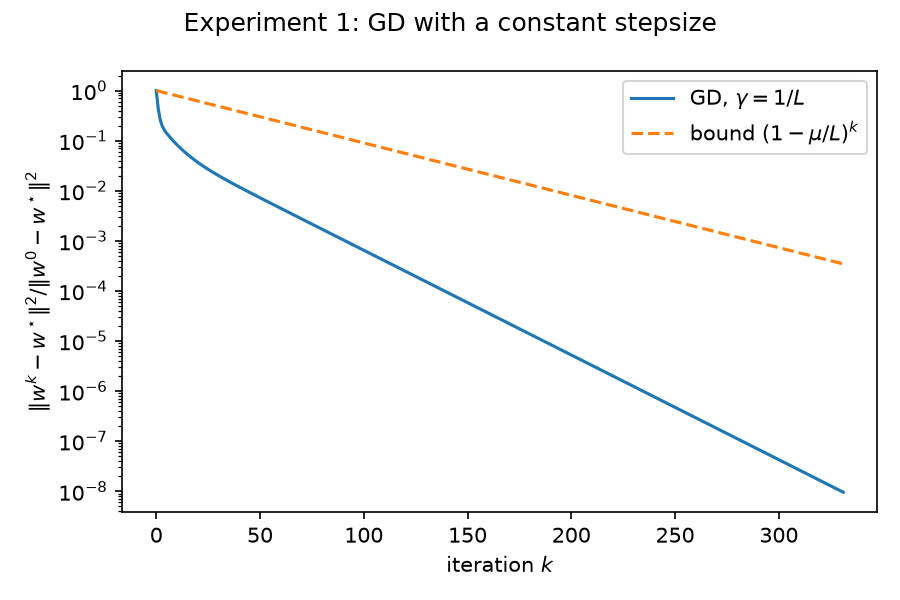
\includegraphics[width=0.6\textwidth]{figures/lin_exp1_gd.png}
\end{center}

The second one is GD with the Polyak stepsize. The plot shows the theoretical bound and the actual convergence,
together with the comparison with the simple GD.

\begin{center}
  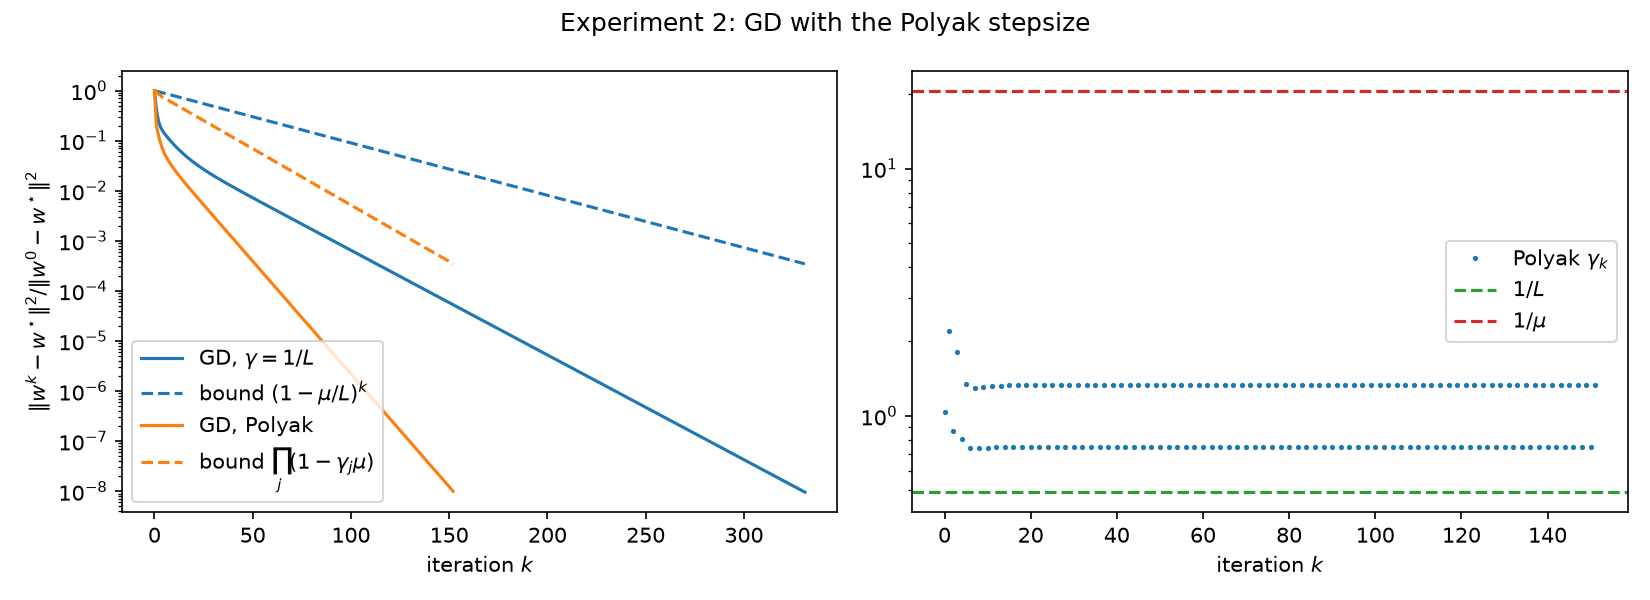
\includegraphics[width=\textwidth]{figures/lin_exp2_polyak.png}
\end{center}

After them come SGD-US and SGD-IS with their theoretical maximal stepsizes $\frac{1}{A}$, and also some experiments
with other stepsizes. They show how the stepsize changes the convergence speed and the size of the neighbourhood,
and what happens when we take a much larger $\gamma$ than the theory allows.

\begin{center}
  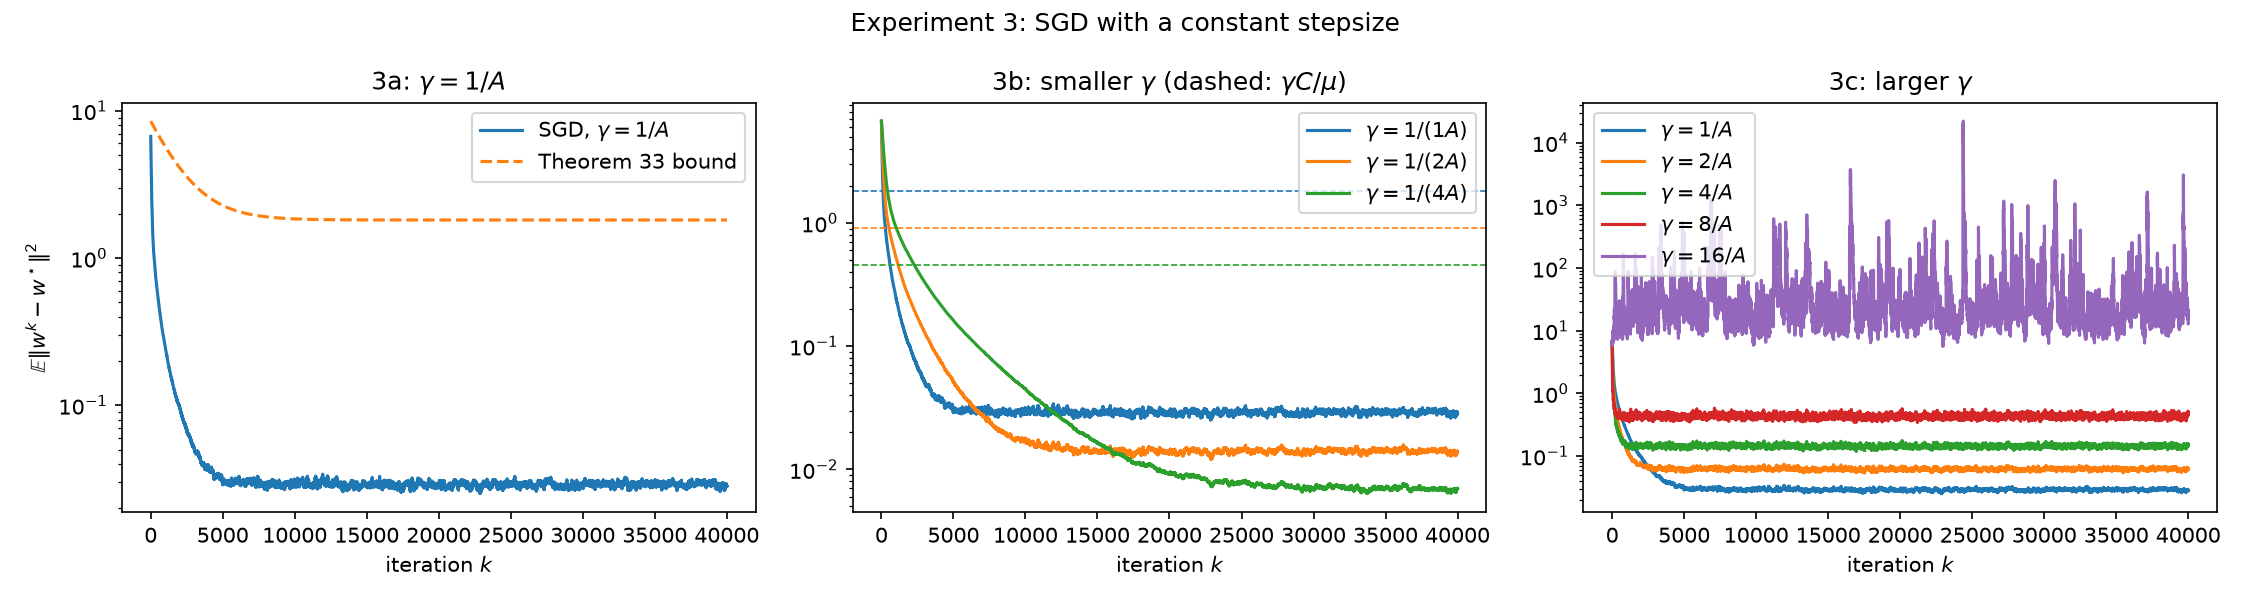
\includegraphics[width=\textwidth]{figures/lin_exp3_sgd.png}
\end{center}

\begin{center}
  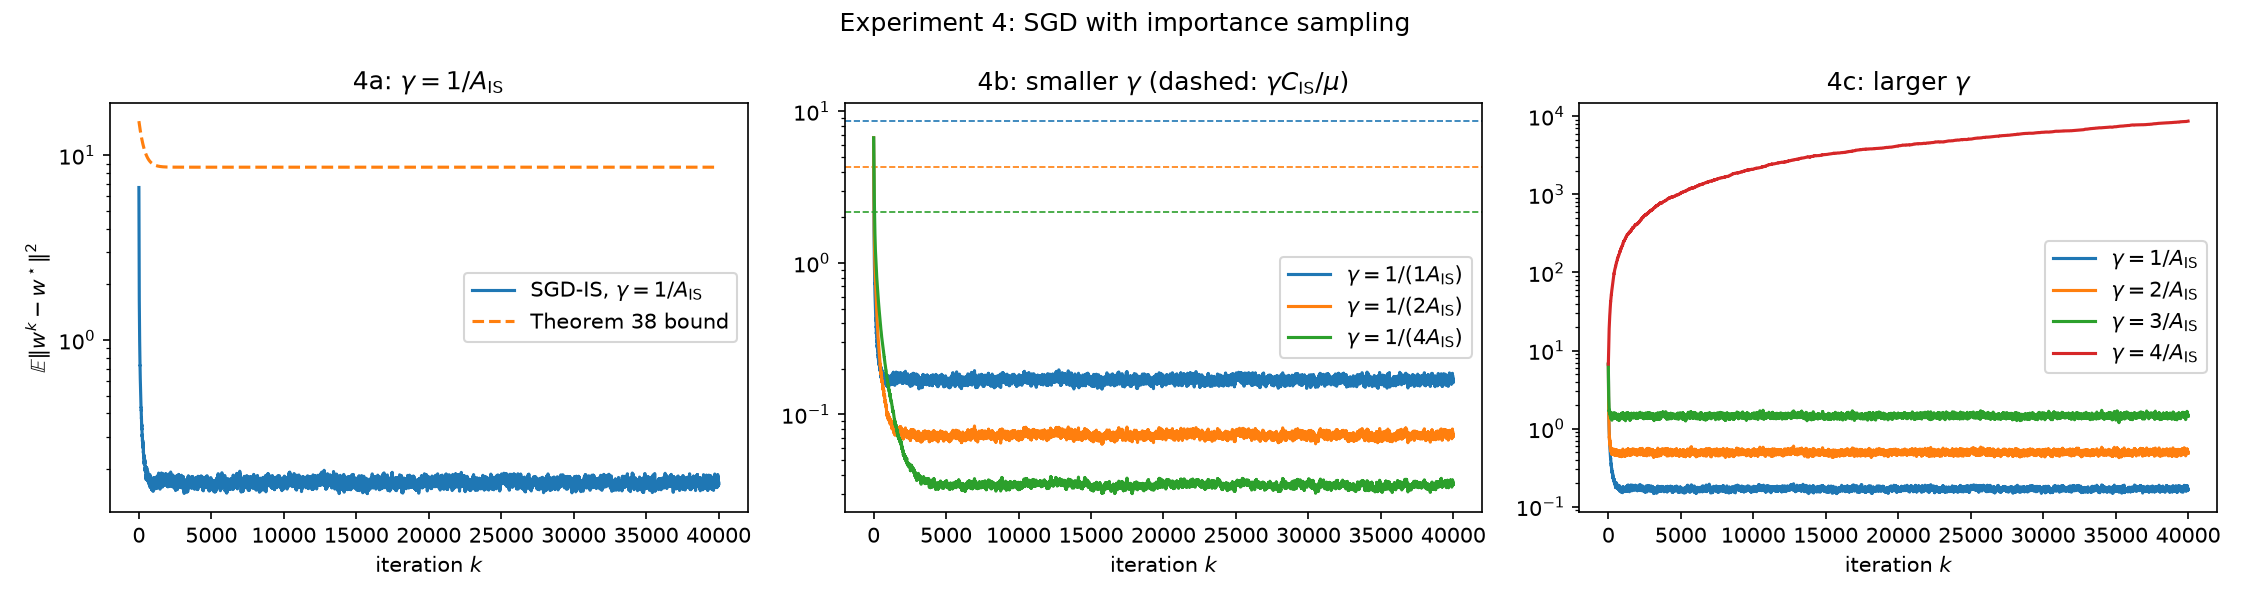
\includegraphics[width=\textwidth]{figures/lin_exp4_sgd_is.png}
\end{center}

\section*{Comparison}

The last experiment is the comparison of all the methods, both by the number of iterations and by the time.

\begin{center}
  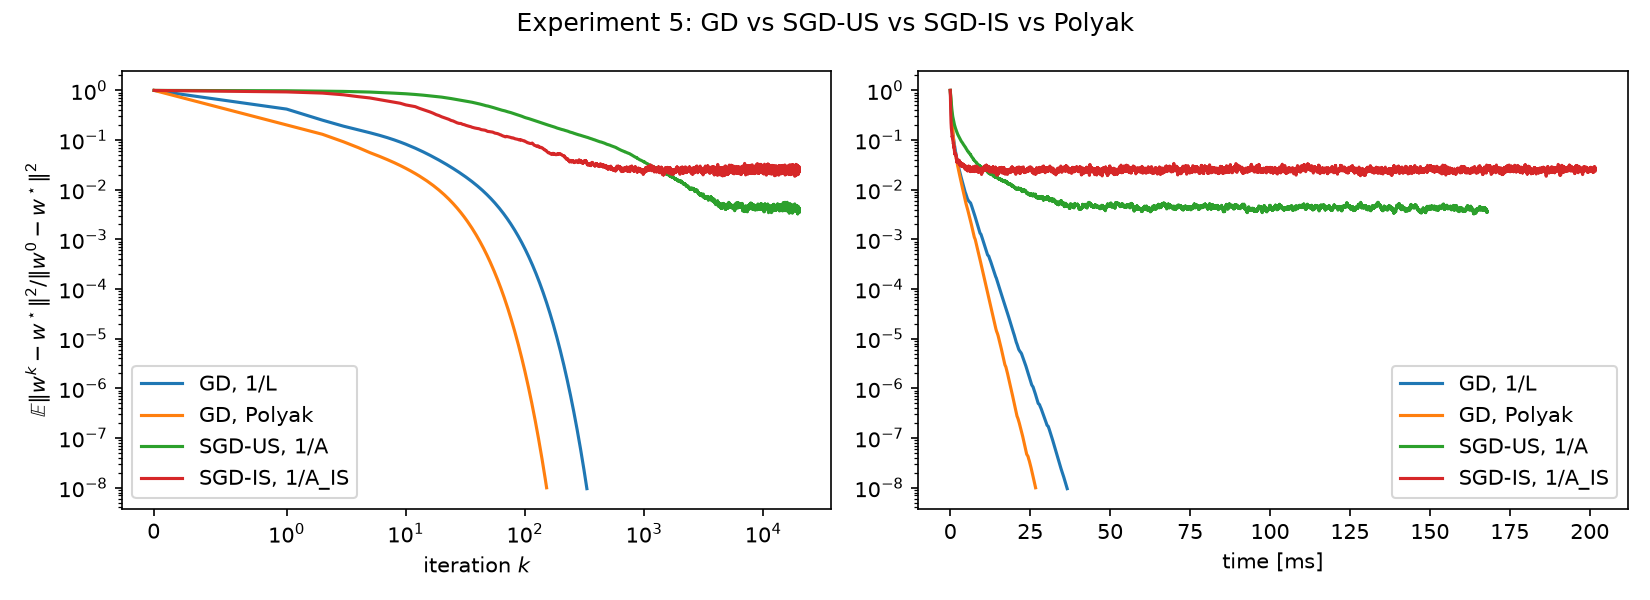
\includegraphics[width=\textwidth]{figures/lin_exp5_comparison.png}
\end{center}

\end{document}
